\documentclass{article}
\usepackage{imports}
\usepackage[russian]{babel}
\usepackage[14pt]{extsizes}
\usepackage{xcolor}
\usepackage{wasysym}
\usepackage{amsmath}
\usepackage{amssymb}
\usepackage{graphicx}
\title{\bfseries Домашняя работа \textnumero 7 по курсу \TeX'а}
\author{Samsonova Varvara}
\date{\today}
\begin{document}
\maketitle
\tableofcontents 
\newpage
\hline\color{blue}\section{Неравенство Йенсена}
$
\hline\color{black}\textbf{Theorem 1.1}(Неравенство Йенсена). Пусть f(x) выпукла вверх на [a,b]. Тогда \forall x_1,...,x_n \in [a,b] и их выпуклой комбинации выполнено неравенство \sum^n_k=1 \alpha_k f(x_k) \leqslant f(\sum^n_{k=1}\alpha_k x_k)
$
\textit{Доказательство.} (Докажем по индукции)
\textbf{База:}n=2
Неравенство превращается в определение выпуклой вверх функции, для которой это, очевидно выполняется.
\textbf{Переход:} Пусть это верно для n. Докажем, что это верно для n+1:
$
~~~~~~~~~~~~~\displaystyle\sum^{n+1}_{k=1} \alpha_k=1, 
$
обозначим зa
$
s_n=\displaystyle\sum^n_{k=1} \alpha_k
пусть \beta_k=\cfrac{\alpha_k}{s_n}.
$
Тогда получаем 
$
\displaystyle\sum^n_{k=1} \beta_k =1
\displaystyle\sum^{n+1}_{k=1} \alpha_k f(x_k)=s_n\displaystyle\sum^n_{k=1} \beta_k f(x_k)+\alpha_n+1 f(x_n+1)  \leqslant $ (по предположению индукции)$ s_n f (\displaystyle\sum^n_{k=1} \beta_k x_k)+ \alpha_{n+1} f(x_{n+1}) \leqslant
$
$\leqslant $( tак кaк $ s_n+\alpha_{n+1}=1) f(\displaystyle\sum^{n+1}_{k=0} \alpha_k x_k)
$
Значит, шаг индукции проделан, неравенство доказано для произвольного n.
\newpage
\hline\color{blue}\section{Круги Эйлера}
\hline\color{black}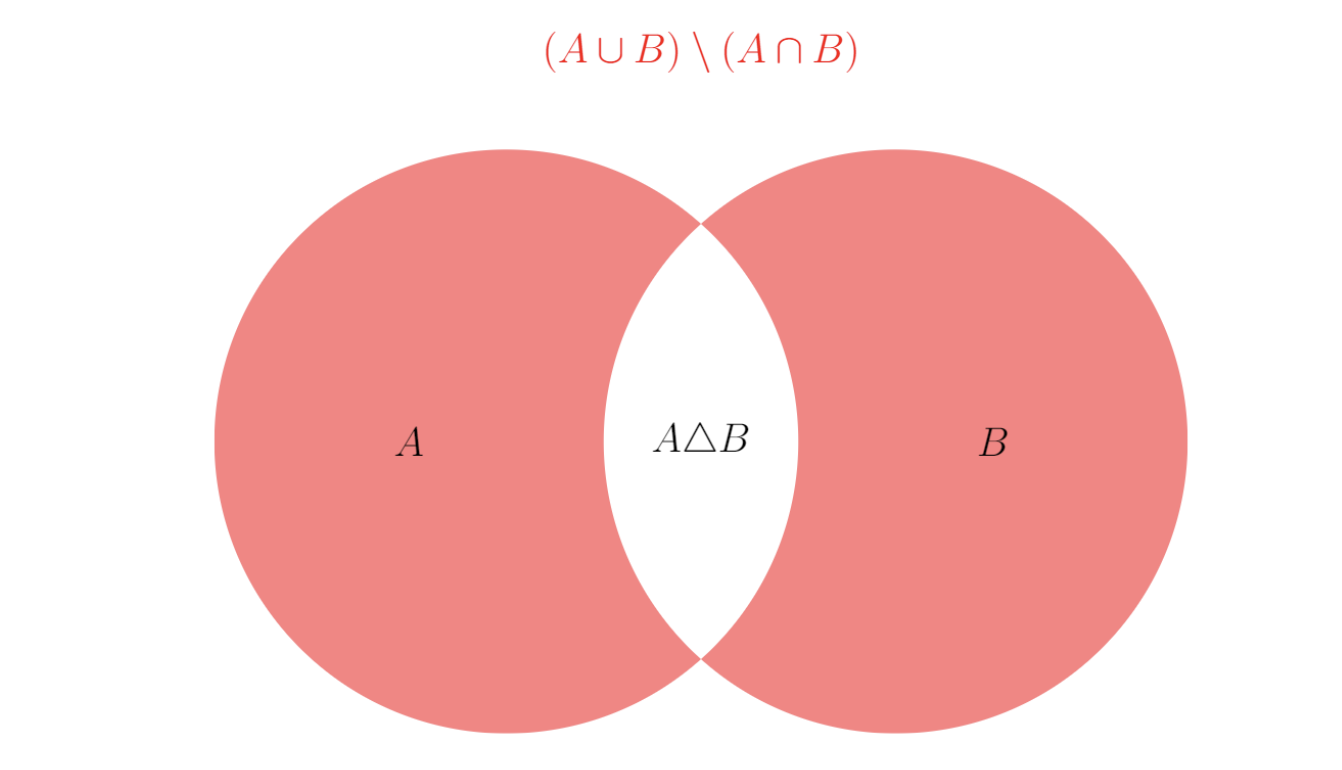
\includegraphics[0.5]{krugieuler.png}
\caption{Pис. 1: круги эйлера}
\end{document}
